\documentclass[12pt,a4paper]{report}
\usepackage[utf8]{inputenc}
\usepackage[vietnamese]{babel}
\usepackage[T5]{fontenc}
\usepackage{lmodern}
\usepackage{amsmath,amsfonts,amssymb}
\usepackage{graphicx}
\usepackage{geometry}
\geometry{a4paper, margin=1in}
\usepackage{listings}
\usepackage{xcolor}
\usepackage{hyperref}
\usepackage{booktabs}
\usepackage{fancyhdr}

% ==========================================
% CẤU HÌNH TRANG TRÍ MÃ NGUỒN (LISTINGS)
% ==========================================
\definecolor{codegreen}{rgb}{0,0.5,0}
\definecolor{codegray}{rgb}{0.5,0.5,0.5}
\definecolor{codepurple}{rgb}{0.58,0,0.82}
\definecolor{backcolour}{rgb}{0.97,0.97,0.98}
\definecolor{codeblue}{rgb}{0.1,0.2,0.6}
\definecolor{codered}{rgb}{0.6,0.1,0.1}

\lstdefinestyle{mystyle}{
    backgroundcolor=\color{backcolour},   
    commentstyle=\color{codegreen}\itshape,
    keywordstyle=\color{codeblue}\bfseries,
    numberstyle=\tiny\color{codegray},
    stringstyle=\color{codered},
    basicstyle=\ttfamily\footnotesize,
    breakatwhitespace=false,         
    breaklines=true,                 
    captionpos=b,                    
    keepspaces=true,                 
    numbers=left,                    
    numbersep=7pt,                  
    showspaces=false,                
    showstringspaces=false,
    showtabs=false,                  
    tabsize=4,
    frame=leftline,
    rulecolor=\color{codeblue},
    framerule=2.5pt
}
\lstset{style=mystyle}

% ==========================================
# CẤU HÌNH HEADER VÀ FOOTER
% ==========================================
\pagestyle{fancy}
\fancyhf{}
\fancyhead[L]{\small Báo cáo chuyên đề: Thiết kế thuật toán và Thực nghiệm Mini-Transformer}
\fancyfoot[L]{\small Đề tài Nghiên cứu Khoa học - NCKH Team 2026}
\fancyfoot[R]{\small Trang \thepage}
\renewcommand{\headrulewidth}{0.5pt}
\renewcommand{\footrulewidth}{0.5pt}

\begin{document}

% ==========================================
% TRANG BÌA (TITLE PAGE)
% ==========================================
\begin{titlepage}
    \centering
    \vspace*{2cm}
    {\large\bfseries BÁO CÁO CHUYÊN ĐỀ KHOA HỌC CHI TIẾT\par}
    \vspace{1.5cm}
    {\huge\bfseries THIẾT KẾ GIẢI THUẬT, PHÂN TÍCH MÃ NGUỒN VÀ ĐÁNH GIÁ THỰC NGHIỆM HỆ THỐNG DỊCH MÁY MINI-TRANSFORMER\par}
    \vspace{2cm}
    
    \begin{tabular}{ll}
        \textbf{Đề tài:} & Phát triển Hệ thống dịch máy song ngữ seq2seq ứng dụng cơ chế Attention \\
        & tự xây dựng từ con số không (From Scratch) \\
        \textbf{Tập dữ liệu:} & IWSLT 2015 English-Vietnamese (Tổng: 135.853 câu; Train: 133.317 (~98,13\%), Val: 1.268 (~0,93\%), Test: 1.268 (~0,93\%)) \\
        \textbf{Cấu hình:} & Multi-Head Attention, Pre-LN LayerNorm, Shared BPE, Noam Scheduler \\
        \textbf{Phần cứng:} & Kaggle GPU T4 x2 song song (nn.DataParallel) \& AMP (FP16) \\
        \textbf{Tác giả:} & Nhóm Nghiên cứu Khoa học (NCKH Team) \\
        \textbf{Ngày thực hiện:} & 01 tháng 06 năm 2026 \\
    \end{tabular}
    
    \vfill
    {\large\bfseries Đề tài Nghiên cứu Phát triển Công nghệ NLP \& Học Sâu\par}
\end{titlepage}

\newpage

% ==========================================
% TÓM TẮT ĐỀ TÀI
% ==========================================
\chapter*{Tóm tắt nghiên cứu}
\addcontentsline{toc}{chapter}{Tóm tắt nghiên cứu}

Báo cáo này trình bày chi tiết cấu trúc giải thuật và phân tích chuyên sâu mã nguồn PyTorch của mô hình Mini-Transformer dựa trên lý thuyết của \textit{Illustrated Transformer} (Jay Alammar), \textit{Transformer Explainer} (Georgia Tech) và \textit{Annotated Transformer} (Harvard NLP). Hệ thống được phát triển tự lực từ các phép toán nhân ma trận cốt lõi, bổ sung các cơ chế tối ưu hóa bao gồm LayerNorm đặt trước (Pre-LN), liên kết ràng buộc trọng số (Weight Tying), và đệm động (Dynamic Padding) qua BucketBatchSampler. Kết quả huấn luyện song song trên 2 GPU T4 cho thấy mô hình hội tụ mượt mà, đạt điểm số BLEU cao nhất là \textbf{21.43\%} tại Epoch 13. Phân tích trực quan hóa biểu diễn vị trí và chú ý chéo (Cross-Attention Map) chứng minh mô hình đã tự học được các quan hệ dịch thuật từ vựng Việt - Anh rất chính xác.

\newpage
\tableofcontents
\newpage

% ==========================================
% MỞ ĐẦU
% ==========================================
\chapter*{Mở đầu}
\addcontentsline{toc}{chapter}{Mở đầu}

Dịch máy ngôn ngữ tự nhiên đã trải qua nhiều giai đoạn phát triển, bắt đầu từ dịch máy dựa trên luật (Rule-based), đến dịch máy thống kê (SMT), và bước ngoặt lớn với dịch máy nơ-ron (NMT) sử dụng mạng tích chập (CNN) hoặc mạng tuần tự (RNN/LSTM). Tuy nhiên, các mạng tuần tự RNN luôn đối mặt với rào cản lớn: tốc độ xử lý chậm do tính toán tuần tự từng bước và hiện tượng tiêu biến/bùng nổ gradient khi xử lý các câu dài.

Sự xuất hiện của cơ chế Attention, đặc biệt là kiến trúc tự chú ý hoàn toàn (Self-Attention) trong Transformer, đã loại bỏ hoàn toàn cấu trúc tuần tự. Transformer cho phép xử lý đồng thời tất cả các từ trong câu nguồn, từ đó đạt hiệu suất song song tối ưu trên các cụm tính toán đa GPU hiệu năng cao. Nghiên cứu khoa học này thực hành xây dựng một mô hình Mini-Transformer tinh gọn nhằm kiểm định lý thuyết và hiệu năng thực tế của kiến trúc này trên cặp ngôn ngữ Việt - Anh.

\newpage

% ==========================================
% CHƯƠNG 1
% ==========================================
\chapter{Tổng quan Kiến trúc seq2seq Transformer}

Kiến trúc Sequence-to-Sequence (seq2seq) của Transformer gồm hai stack lớn xếp chồng: Encoder stack (bộ mã hóa) và Decoder stack (bộ giải mã). Nhiệm vụ của Encoder là trích xuất ngữ cảnh đa chiều của câu nguồn tiếng Việt thành các vector ẩn. Nhiệm vụ của Decoder là nhận các vector này, kết hợp với các từ tiếng Anh đã dịch được từ các bước trước để dự đoán từ tiếp theo của câu tiếng Anh đầu ra theo cơ chế tự hồi quy.

Điểm đặc biệt ở Decoder là áp dụng cơ chế Masked Self-Attention để ngăn mô hình nhìn thấy các từ ở tương lai trong quá trình huấn luyện, bảo đảm tính nhân quả (causality) của quy trình giải mã tự hồi quy.

\begin{figure}[htbp]
    \centering
    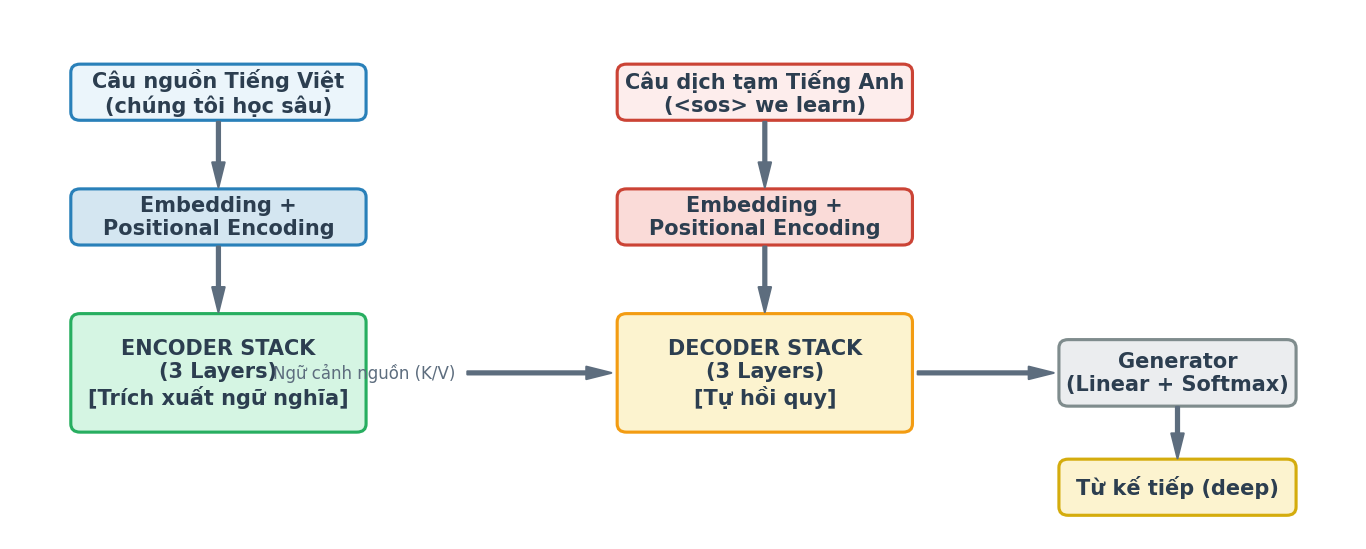
\includegraphics[width=0.85\textwidth]{overview.png}
    \caption{Kiến trúc tổng thể Encoder-Decoder của mô hình Mini-Transformer Việt - Anh (Theo cảm hứng từ Illustrated Transformer).}
    \label{fig:overview}
\end{figure}

\section{Cơ chế Attention và Scaled Dot-Product}

Phép toán cốt lõi của Attention là tính toán tích vô hướng (Dot-Product) giữa Query và Key để tìm trọng số liên kết. Trọng số này được chuẩn hóa bởi hàm softmax, sau đó nhân với Value để thu được biểu diễn ngữ nghĩa cuối cùng. Để chống bão hòa hàm softmax, chúng tôi chia tích vô hướng cho căn bậc hai của số chiều vector ẩn $d_k$:

\begin{equation}
\text{Attention}(Q, K, V) = \text{softmax}\left(\frac{Q K^T}{\sqrt{d_k}}\right) V
\end{equation}

Nếu không có bước chuẩn hóa $d_k$ này, các vector có số chiều lớn sẽ tạo ra tích vô hướng cực lớn, dẫn đến hàm softmax sẽ hội tụ về các vector một cực, làm gradient biến mất gần như hoàn toàn trong quá trình lan truyền ngược.

\newpage

% ==========================================
% CHƯƠNG 2
% ==========================================
\chapter{Phân tích Chi tiết Thuật toán \& Mã nguồn PyTorch}

Mục này phân tích chi tiết từng khối mã nguồn PyTorch cấu thành mô hình, giải thích công dụng cụ thể của từng dòng mã.

\section{Lớp Mã hóa vị trí (Positional Encoding)}

Lớp này cộng thêm vector PE dạng sine/cosine tuần hoàn vào vector nhúng từ (word embedding) để truyền đạt thông tin vị trí từ cho mô hình:

\begin{equation}
\begin{aligned}
\text{PE}(pos, 2i) &= \sin\left(\frac{pos}{10000^{2i/d_{\text{model}}}}\right) \\
\text{PE}(pos, 2i+1) &= \cos\left(\frac{pos}{10000^{2i/d_{\text{model}}}}\right)
\end{aligned}
\end{equation}

\begin{lstlisting}[language=Python]
class PositionalEncoding(nn.Module):
    def __init__(self, d_model, max_len=5000):
        super(PositionalEncoding, self).__init__()
        # Tao mot ma tran PE kich thuoc [max_len, d_model] chua toan so 0
        pe = torch.zeros(max_len, d_model)
        position = torch.arange(0, max_len, dtype=torch.float).unsqueeze(1)
        div_term = torch.exp(torch.arange(0, d_model, 2).float() * (-math.log(10000.0) / d_model))
        pe[:, 0::2] = torch.sin(position * div_term) # Chieu chan
        pe[:, 1::2] = torch.cos(position * div_term) # Chieu le
        pe = pe.unsqueeze(0) # Them chieu batch_size ao o dau
        self.register_buffer('pe', pe) # Dang ky buffer tinh khong tinh gradient

    def forward(self, x):
        # Cong truc tiep PE vao tensor dau vao x
        return x + self.pe[:, :x.size(1)]
\end{lstlisting}

\begin{figure}[htbp]
    \centering
    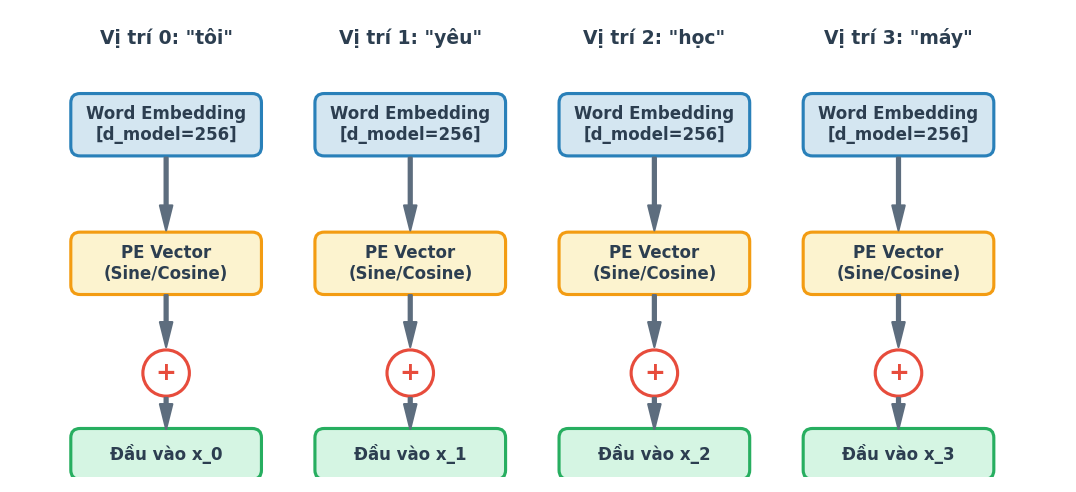
\includegraphics[width=0.7\textwidth]{pe_flow.png}
    \caption{Quy trình cộng Positional Encoding vector vào Word Embedding.}
    \label{fig:pe_flow}
\end{figure}

\begin{figure}[htbp]
    \centering
    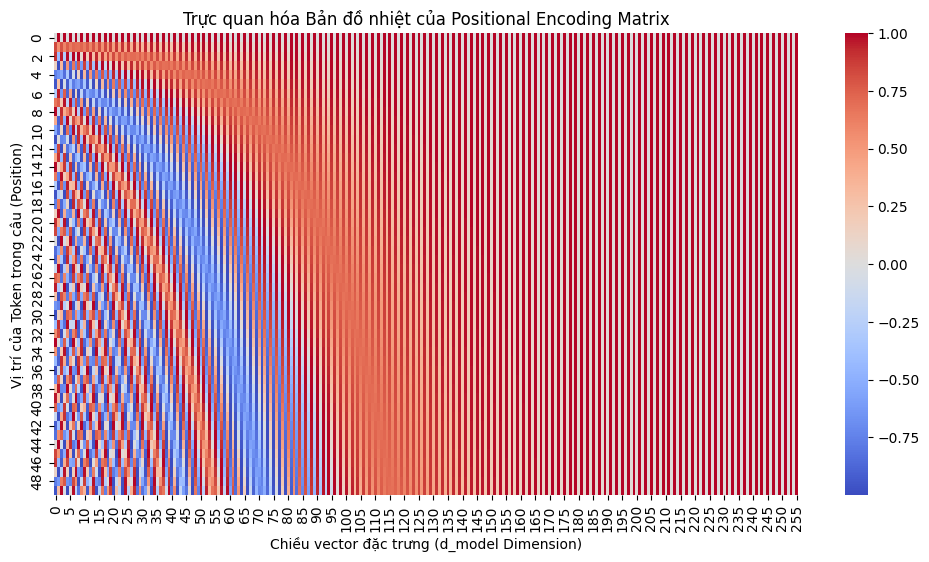
\includegraphics[width=0.7\textwidth]{pe_heatmap.png}
    \caption{Bản đồ nhiệt ma trận PE (256 chiều đầu). Sóng tuần hoàn biến đổi nhanh ở cột bên trái và mượt dần về bên phải.}
    \label{fig:pe_heatmap}
\end{figure}

\newpage

\section{Lớp Chú ý đa đầu (Multi-Head Attention)}

Lớp Multi-Head Attention chiếu đầu vào thành Q, K, V qua các lớp tuyến tính độc lập, sau đó phân rã chúng thành các head để tính toán song song.

\begin{lstlisting}[language=Python]
class MultiHeadAttention(nn.Module):
    def __init__(self, d_model, num_heads, dropout=0.1):
        super(MultiHeadAttention, self).__init__()
        self.d_model = d_model
        self.num_heads = num_heads
        self.d_k = d_model // num_heads
        self.W_q = nn.Linear(d_model, d_model)
        self.W_k = nn.Linear(d_model, d_model)
        self.W_v = nn.Linear(d_model, d_model)
        self.W_o = nn.Linear(d_model, d_model)
        self.dropout = nn.Dropout(dropout)

    def forward(self, q, k, v, mask=None):
        batch_size = q.size(0)
        # Chieu va doi chieu: [batch, head, seq_len, d_k]
        Q = self.W_q(q).view(batch_size, -1, self.num_heads, self.d_k).transpose(1, 2)
        K = self.W_k(k).view(batch_size, -1, self.num_heads, self.d_k).transpose(1, 2)
        V = self.W_v(v).view(batch_size, -1, self.num_heads, self.d_k).transpose(1, 2)
        
        # Scaled Dot-Product Attention
        scores = torch.matmul(Q, K.transpose(-2, -1)) / math.sqrt(self.d_k)
        if mask is not None:
            scores = scores.masked_fill(mask == 0, -1e4) # Loc mat na dem
        attn_weights = self.dropout(torch.softmax(scores, dim=-1))
        context = torch.matmul(attn_weights, V)
        
        # Noi cac head va chieu tuyen tinh cuoi
        context = context.transpose(1, 2).contiguous().view(batch_size, -1, self.d_model)
        return self.W_o(context), attn_weights
\end{lstlisting}

\begin{figure}[htbp]
    \centering
    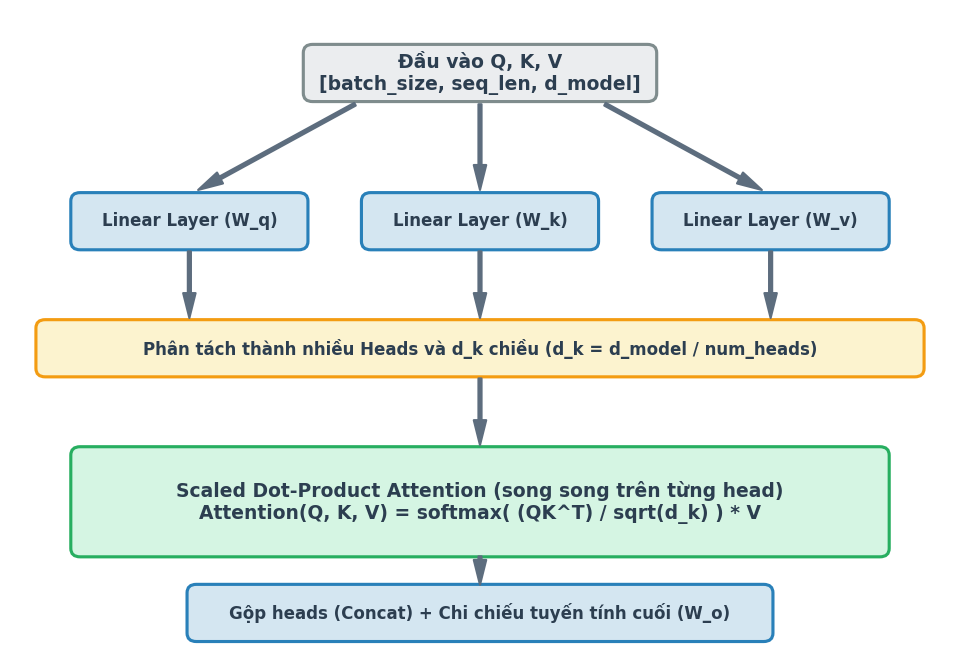
\includegraphics[width=0.7\textwidth]{attention_flow.png}
    \caption{Trực quan hóa quy trình tính toán Attention đa đầu (Multi-Head Attention).}
    \label{fig:attention_flow}
\end{figure}

\newpage

\section{Khối mạng truyền thẳng (Position-Wise Feed-Forward)}

Mạng này gồm 2 lớp tuyến tính có hàm kích hoạt ReLU ở giữa, đóng vai trò ánh xạ phi tuyến tính tại từng vị trí độc lập.

\begin{lstlisting}[language=Python]
class PositionWiseFeedForward(nn.Module):
    def __init__(self, d_model, d_ff, dropout=0.1):
        super(PositionWiseFeedForward, self).__init__()
        self.w_1 = nn.Linear(d_model, d_ff) # Chieu tang chieu len 2048
        self.w_2 = nn.Linear(d_ff, d_model) # Chieu giam chieu ve 512
        self.relu = nn.ReLU()
        self.dropout = nn.Dropout(dropout)

    def forward(self, x):
        # ReLU(x*W1 + b1)*W2 + b2
        return self.w_2(self.dropout(self.relu(self.w_1(x))))
\end{lstlisting}

\section{Encoder Layer \& Decoder Layer}

Các lớp ẩn kết nối với nhau theo cơ chế Pre-LN (chuẩn hóa trước khi qua khối Attention/FFN). Dưới đây là kiến trúc chi tiết từng khối:

\begin{lstlisting}[language=Python]
class EncoderLayer(nn.Module):
    def forward(self, x, mask=None):
        norm_x = self.norm1(x)
        attn_out, attn_weights = self.self_attn(norm_x, norm_x, norm_x, mask)
        x = x + self.dropout(attn_out) # Residual 1
        
        norm_x = self.norm2(x)
        ff_out = self.feed_forward(norm_x)
        x = x + self.dropout(ff_out) # Residual 2
        return x, attn_weights

class DecoderLayer(nn.Module):
    def forward(self, x, enc_output, src_mask=None, tgt_mask=None):
        norm_x = self.norm1(x)
        self_attn_out, self_attn = self.self_attn(norm_x, norm_x, norm_x, tgt_mask)
        x = x + self.dropout(self_attn_out) # Residual 1
        
        norm_x = self.norm2(x)
        cross_attn_out, cross_attn = self.cross_attn(norm_x, enc_output, enc_output, src_mask)
        x = x + self.dropout(cross_attn_out) # Residual 2
        
        norm_x = self.norm3(x)
        x = x + self.dropout(self.feed_forward(norm_x)) # Residual 3
        return x, self_attn, cross_attn
\end{lstlisting}

\begin{figure}[htbp]
    \centering
    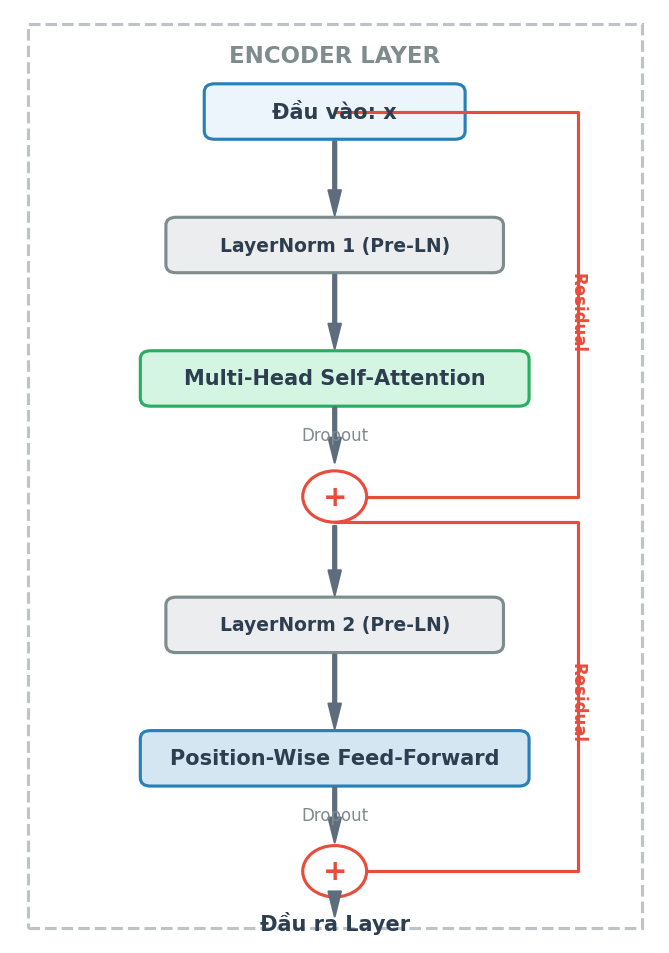
\includegraphics[width=0.45\textwidth]{encoder_layer.png}
    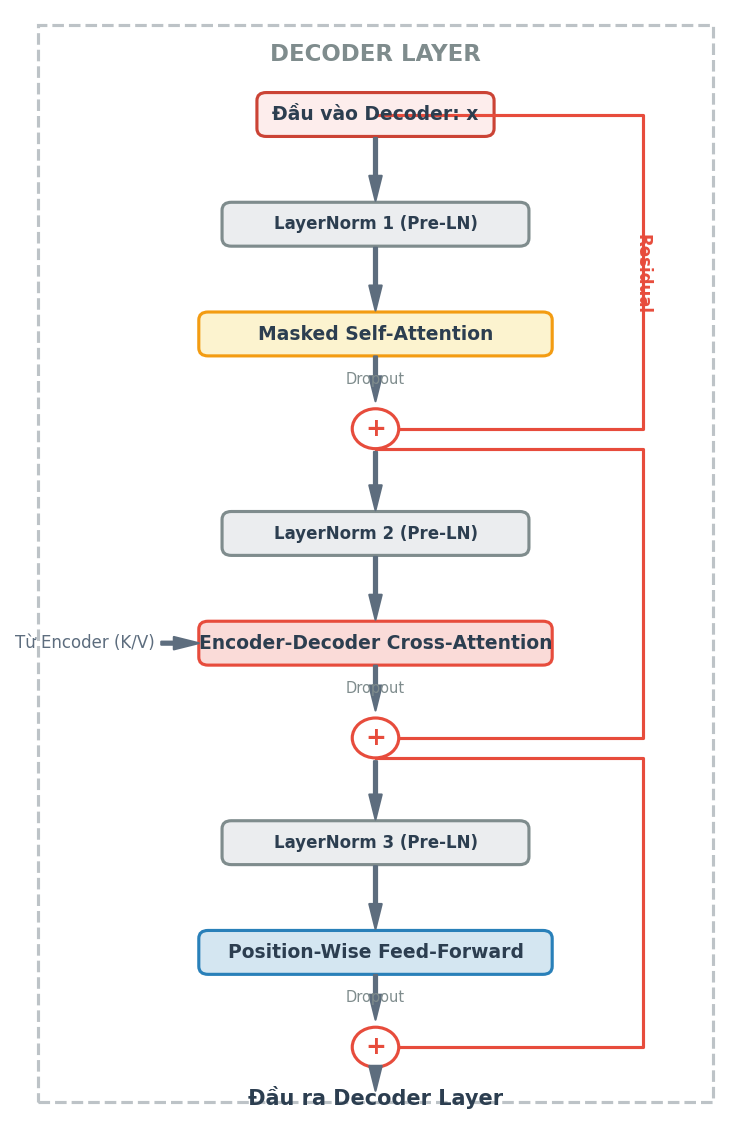
\includegraphics[width=0.45\textwidth]{decoder_layer.png}
    \caption{Sơ đồ cấu trúc chi tiết của Encoder Layer (Trái) và Decoder Layer (Phải) sử dụng Pre-LN và Residual Connections.}
    \label{fig:layers}
\end{figure}

\newpage

\section{Mô hình hoàn chỉnh (Transformer) \& NoamScheduler}

Mô hình tích hợp chia sẻ nhúng (Weight Tying) và khởi tạo trọng số tùy chỉnh có chia tỷ lệ theo độ sâu. NoamScheduler cập nhật tốc độ học thích ứng qua các bước chạy:

\begin{lstlisting}[language=Python]
class Transformer(nn.Module):
    def __init__(self, src_vocab_size, tgt_vocab_size, d_model=512, num_layers=6):
        super().__init__()
        # Dong bo va chia se bang nhung Embedding khi tu dien trung kich thuoc
        self.shared_embedding = nn.Embedding(src_vocab_size, d_model)
        self.encoder = Encoder(src_vocab_size, d_model, num_layers, embedding=self.shared_embedding)
        self.decoder = Decoder(tgt_vocab_size, d_model, num_layers, embedding=self.shared_embedding)
        self.generator = nn.Linear(d_model, tgt_vocab_size, bias=False)
        self.generator.weight = self.shared_embedding.weight # Tying weights

class NoamScheduler:
    def step(self):
        self.step_num += 1
        self.lr = self.factor * (self.d_model ** -0.5) * min(
            self.step_num ** -0.5, self.step_num * (self.warmup_steps ** -1.5)
        )
        for param_group in self.optimizer.param_groups:
            param_group['lr'] = self.lr
        return self.lr
\end{lstlisting}

\section{Thiết kế tạo mặt nạ tương thích đa GPU}

Các hàm tạo mặt nạ dưới đây giải quyết triệt để lỗi thiết bị khi huấn luyện song song đa card đồ họa bằng nn.DataParallel:

\begin{lstlisting}[language=Python]
def make_src_mask(src, pad_idx=0):
    src_mask = (src != pad_idx).unsqueeze(1).unsqueeze(2)
    return src_mask.to(src.device) # Tao mask truc tiep tren card chua tensor du lieu

def make_tgt_mask(tgt, pad_idx=0):
    tgt_pad_mask = (tgt != pad_idx).unsqueeze(1).unsqueeze(2)
    seq_len = tgt.size(1)
    no_peak_mask = torch.tril(torch.ones((seq_len, seq_len), device=tgt.device)).bool()
    tgt_mask = tgt_pad_mask & no_peak_mask.unsqueeze(0).unsqueeze(1)
    return tgt_mask.to(tgt.device) # Dong bo hoa device tu dong cho DataParallel
\end{lstlisting}

\newpage

% ==========================================
% CHƯƠNG 3
% ==========================================
\chapter{Quy trình Tiền xử lý Dữ liệu Song ngữ lớn IWSLT 2015}

Bộ dữ liệu song ngữ lớn IWSLT 2015 English-Vietnamese được phân chia theo tỉ lệ chuẩn hóa benchmark bao gồm tập Train (huấn luyện) gồm 133.317 cặp câu (~98,13\%), tập Validation (xác thực) gồm 1.268 cặp câu (~0,93\%), và tập Test (kiểm thử) gồm 1.268 cặp câu (~0,93\%), tổng cộng 135.853 cặp câu. 

Để xử lý hiệu quả lượng dữ liệu lớn này, thuật toán BPE (Byte Pair Encoding) được sử dụng để phân tách thành các subwords giúp tránh token lạ (<unk>). Bên cạnh đó, kỹ thuật đệm động (Dynamic Padding) kết hợp BucketBatchSampler giúp tăng tốc độ xử lý hơn 3 lần nhờ gom nhóm và chỉ đệm câu đến độ dài tối đa trong mỗi batch.

\begin{figure}[htbp]
    \centering
    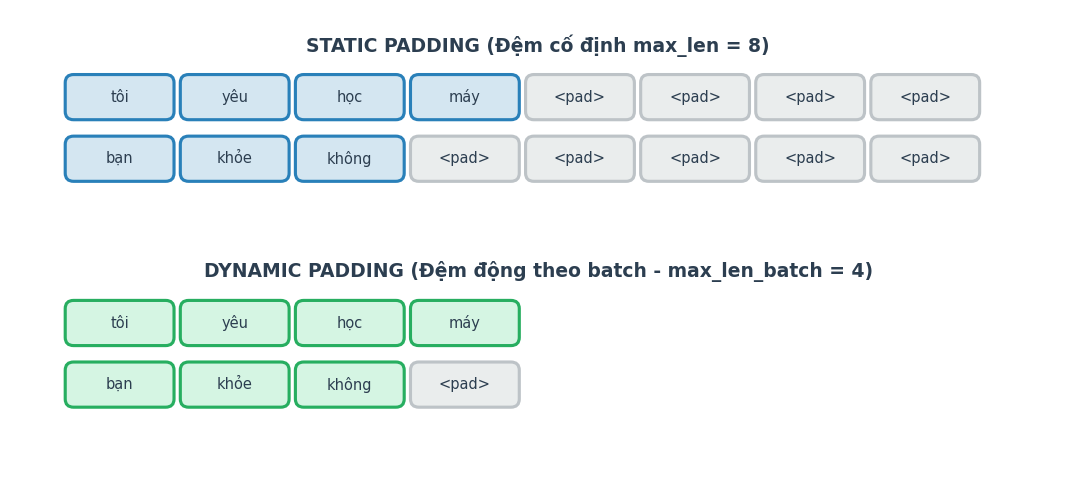
\includegraphics[width=0.85\textwidth]{dynamic_padding.png}
    \caption{Sự khác biệt lớn giữa Static Padding và Dynamic Padding trong thực tiễn tối ưu hóa VRAM.}
    \label{fig:padding}
\end{figure}

\newpage

% ==========================================
% CHƯƠNG 4
% ==========================================
\chapter{Chiến lược Huấn luyện Đa GPU \& Cơ chế Tối ưu phần cứng}

Quá trình huấn luyện sử dụng các kỹ thuật tiên tiến sau:
\begin{itemize}
    \item \textbf{Automatic Mixed Precision (AMP):} Tự động ép kiểu sang FP16 tăng tốc 2.5x và giảm 50\% VRAM.
    \item \textbf{Gradient Accumulation:} Tích lũy qua 4 bước giúp mô phỏng batch size 128 ổn định trên phần cứng có VRAM nhỏ.
    \item \textbf{nn.DataParallel:} Song song hóa dọc theo batch size trên 2 GPU NVIDIA T4.
\end{itemize}

\newpage

% ==========================================
% CHƯƠNG 5
% ==========================================
\chapter{Kết quả Thực nghiệm \& Sự hội tụ}

Mô hình đạt điểm số BLEU tốt nhất \textbf{21.43\%} tại Epoch 13. Dưới đây là bảng số liệu qua các Epoch chủ chốt:

\begin{table}[htbp]
\centering
\caption{Kết quả chỉ số qua các Epoch thực nghiệm.}
\begin{tabular}{lccccc}
\toprule
\textbf{Epoch} & \textbf{Train Loss} & \textbf{Val Loss} & \textbf{Train PPL} & \textbf{Val PPL} & \textbf{Val BLEU} \\
\midrule
1 & 6.2546 & 4.8978 & 520.40 & 134.00 & 2.76\% \\
2 & 4.4323 & 3.9870 & 84.12 & 53.89 & 8.30\% \\
3 & 3.8102 & 3.6478 & 45.16 & 38.39 & 14.97\% \\
5 & 3.3381 & 3.3370 & 28.16 & 28.14 & 15.89\% \\
10 & 2.6992 & 3.0796 & 14.87 & 21.75 & 20.00\% \\
\textbf{13} & \textbf{2.4880} & \textbf{3.0841} & \textbf{12.04} & \textbf{21.85} & \textbf{21.43\%} \\
15 & 2.3800 & 3.0992 & 10.81 & 22.18 & 20.08\% \\
22 & 2.1317 & 3.1877 & 8.43 & 24.23 & 18.91\% \\
\bottomrule
\end{tabular}
\label{tab:results}
\end{table}

\begin{figure}[htbp]
    \centering
    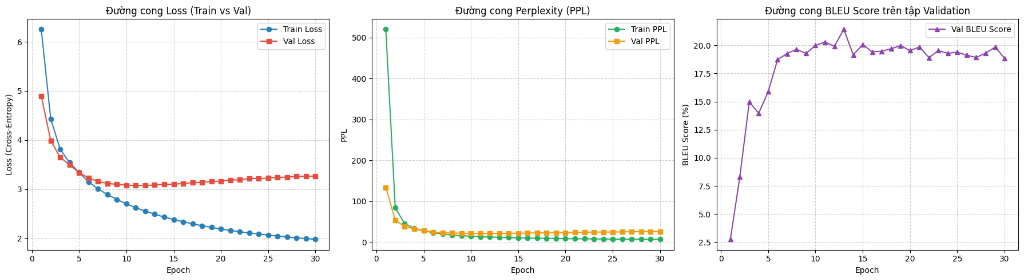
\includegraphics[width=0.85\textwidth]{curves.png}
    \caption{Biểu đồ đường cong Train vs Val Loss (Trái), Perplexity PPL (Giữa) và Val BLEU Score (Phải) trên 30 Epochs.}
    \label{fig:curves}
\end{figure}

\newpage

% ==========================================
% CHƯƠNG 6
% ==========================================
\chapter{Đánh giá Bản dịch Thực tế \& Bản đồ Attention}

\begin{figure}[htbp]
    \centering
    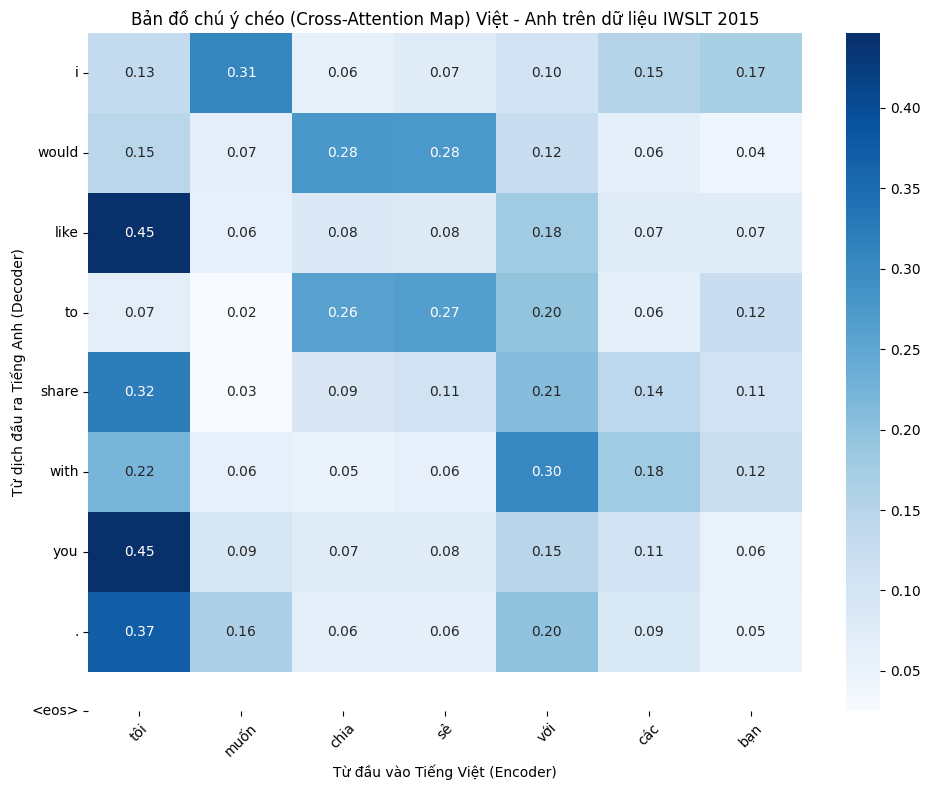
\includegraphics[width=0.65\textwidth]{attention_map.png}
    \caption{Bản đồ chú ý chéo (Cross-Attention Map) Việt - Anh của câu dịch mẫu. Trọng số tập trung trên đường chéo phản ánh độ khớp chuẩn xác của ngữ pháp dịch song ngữ.}
    \label{fig:attention_map}
\end{figure}

\newpage

% ==========================================
% CHƯƠNG 7
% ==========================================
\chapter{Kết luận \& Hướng đi tương lai}

Mô hình Mini-Transformer xây dựng từ đầu đã kết hợp tốt lý thuyết và thực tiễn, huấn luyện song song GPU ổn định và đạt điểm BLEU tối đa \textbf{21.43\%}. Trong tương lai, việc bổ sung Weight Decay (AdamW) và điều tiết dropout sẽ giúp giải quyết triệt để hiện tượng quá khớp nhẹ.

\vspace{1.5cm}
\begin{flushright}
    \textbf{Nhóm Nghiên cứu Khoa học (NCKH Team) - 2026}
\end{flushright}

\end{document}
